\tikzset{every picture/.style={line width=0.75pt}} %set default line width to 0.75pt        

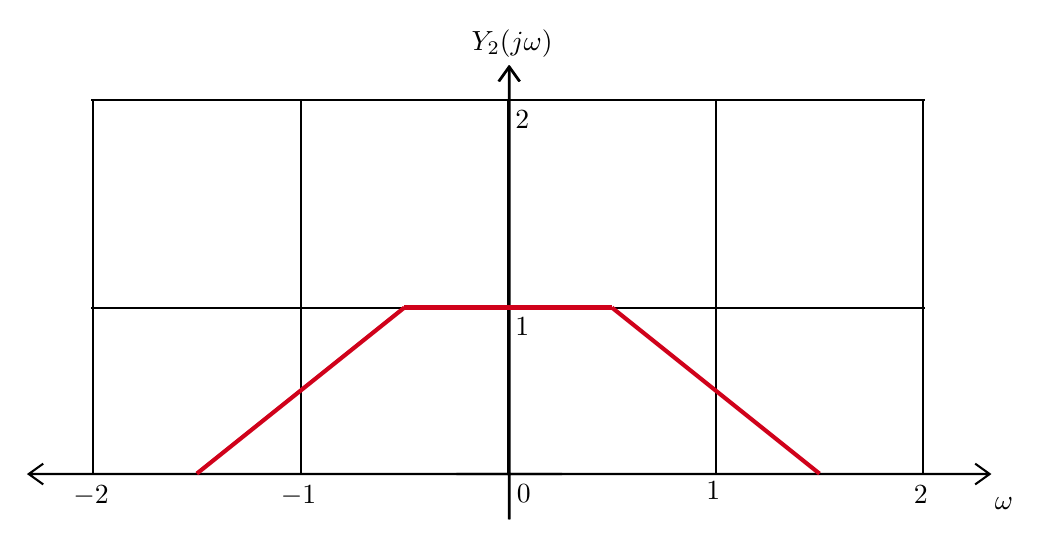
\begin{tikzpicture}[x=0.75pt,y=0.75pt,yscale=-1,xscale=1]
%uncomment if require: \path (0,590); %set diagram left start at 0, and has height of 590

%Shape: Axis 2D [id:dp039547207268332385] 
\draw  (277,252.2) -- (534,252.2)(302.7,56) -- (302.7,274) (527,247.2) -- (534,252.2) -- (527,257.2) (297.7,63) -- (302.7,56) -- (307.7,63)  ;
%Shape: Grid [id:dp9841770007230126] 
\draw  [draw opacity=0] (302,72) -- (503,72) -- (503,252) -- (302,252) -- cycle ; \draw   (302,72) -- (302,252)(402,72) -- (402,252)(502,72) -- (502,252) ; \draw   (302,72) -- (503,72)(302,172) -- (503,172) ; \draw    ;
%Shape: Axis 2D [id:dp9362667242858227] 
\draw  (328,252.2) -- (71,252.2)(302.3,56) -- (302.3,274) (78,247.2) -- (71,252.2) -- (78,257.2) (307.3,63) -- (302.3,56) -- (297.3,63)  ;
%Shape: Grid [id:dp6769124018924975] 
\draw  [draw opacity=0] (302,72) -- (101,72) -- (101,252) -- (302,252) -- cycle ; \draw   (302,72) -- (302,252)(202,72) -- (202,252)(102,72) -- (102,252) ; \draw   (302,72) -- (101,72)(302,172) -- (101,172) ; \draw    ;
%Straight Lines [id:da3649524076190428] 
\draw [color={rgb, 255:red, 208; green, 2; blue, 27 }  ,draw opacity=1 ][line width=1.5]    (252,172) -- (352,172) ;
%Straight Lines [id:da044228377793803286] 
\draw [color={rgb, 255:red, 208; green, 2; blue, 27 }  ,draw opacity=1 ][line width=1.5]    (152,252) -- (252,172) ;
%Straight Lines [id:da9643733463980907] 
\draw [color={rgb, 255:red, 208; green, 2; blue, 27 }  ,draw opacity=1 ][line width=1.5]    (452,252) -- (352,172) ;

% Text Node
\draw (304,175.4) node [anchor=north west][inner sep=0.75pt]    {$1$};
% Text Node
\draw (304,75.4) node [anchor=north west][inner sep=0.75pt]    {$2$};
% Text Node
\draw (396,254.4) node [anchor=north west][inner sep=0.75pt]    {$1$};
% Text Node
\draw (496,256.4) node [anchor=north west][inner sep=0.75pt]    {$2$};
% Text Node
\draw (191,256.4) node [anchor=north west][inner sep=0.75pt]    {$-1$};
% Text Node
\draw (91,256.4) node [anchor=north west][inner sep=0.75pt]    {$-2$};
% Text Node
\draw (304.7,255.6) node [anchor=north west][inner sep=0.75pt]    {$0$};
% Text Node
\draw (303.9,52.98) node [anchor=south] [inner sep=0.75pt]    {$Y_{2}( j\omega )$};
% Text Node
\draw (540.9,270.98) node [anchor=south] [inner sep=0.75pt]    {$\omega $};


\end{tikzpicture}
